\Chapter{Introduction}
\label{Introduction}
\begin{refsection}

\section{Fondamentaux et échelles caractéristiques}
\emph{Le plasma}. Le plasma est souvent considéré un peu équivoquement comme le
quatrième état de la matière. Dans notre environnement proche, nous avons pris
conscience de son existence à travers les phénomènes de flammes, d'éclairs,
d'aurore boréales ou d'arc électriques. Mais à des conditions de pressions et de
températures différentes de celles de notre atmosphère terrestre, il est
omniprésent : plus de 99\% de la matière connue est sous cette forme.

Une définition plus adaptée du plasma est celle d'un gaz conducteur. Une partie
des atomes le composant est ionisée, donnant naissance à une population
d'électrons libres et d'ions de différentes espèces. Ces populations permettent
alors le transport de courant et, sensibles aux forces électromagnétiques,
influencent fortement le comportement global du plasma en provoquant des
phénomènes collectifs, non-linéaires et turbulents.

Le plasma et son comportement sont décrits par la théorie de la physique des
plasmas. Elle intègre les connaissances de nombreux domaines, tels que la
physique statitique, l'électromagnétisme, ou encore la dynamique des fluides.

\subsection{Les paramètres plasmas}
Les plasmas se présentent donc comme des gaz dont le comportement est influencé
de manière non négligeable par une population d'électrons libres. Cette population
se caractérise par deux paramètres principaux :

\begin{itemize}
  \item sa densité, $n_e$, mesurant le nombre de particules par élément de volume
  \item sa température électronique $T_e$, mesurée en électronvolts, représentative
   de l'energie cinétique moyenne non dirigée des électrons (aussi appelée
   agitation thermique)
\end{itemize}

\begin{equation}
	eT_\text{e}=m_\text{e} v_{\text{T}_\text{e}}\puissance{2}
\end{equation}

où $m_\text{e}$ est la masse de l'électron, et $e$ la charge élémentaire. Pour un électron possédant
une énergie de \unit{1}{\electronvolt}, la vitesse thermique est de l'ordre de
\unit{400}{\kilo\meter}.$s\puissance{-1}$.
Du fait de la différence de masse, cette vitesse est bien inférieure pour les
ions, qui à même énergie auront une vitesse thermique d'environ \unit{10}{\kilo\meter}.$s\puissance{-1}$.

\begin{equation}
	v_{\text{T}_\text{i}}\approx\left(m_\text{e}/m_\text{i}\right)^{\text{\textonehalf}}
	v_{\text{T}_\text{e}}
\end{equation}

La figure (\ref{zoologie}) représente une classification des plasmas
en fonction de ces deux paramètres principaux qui vont influer sur la dynamique du
transport des particules et du courant.
La théorie présentée dans la suite de cette thèse ne concerne que les plasmas
dits classiques :

\begin{itemize}
  \item les plasmas naturels peu dense tels que l'espace interstellaire,
  le vent solaire, la magnétosphère, et l'ionosphère
  \item les plasmas naturels denses tels que les éclairs et les étoiles
  \item les plasmas industriels, de laboratoire, et thermonucléaires
\end{itemize}
\begin{figure}[htbp]
\centering
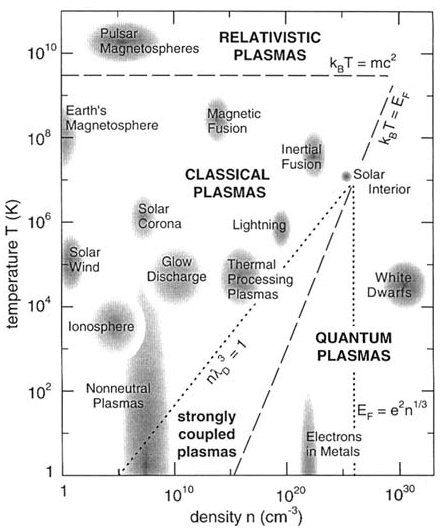
\includegraphics[height=80mm,width=64mm]{figures/zoologie.png}{\caption{Classification
de différents plasmas en fonction de $n_e$ et $T_e$ issue du livre du National
Research Council \parencite{NRC}}\label{zoologie}}
\end{figure}

Dans ces plasmas, le dégré d'ionisation $\alpha$ est donné par le rapport
entre la densité électronique $n_\text{e}$ et la densité de gaz neutre
$n_\text{n}$ :

\begin{equation}
\alpha=\frac{n_\text{e}}{n_\text{e}+n_\text{n}}
\end{equation}

Cette fraction va définir l'importance de l'interaction entre les particules
neutres et les particules chargées. Cependant, même à très faible $\alpha$,
l'apparition d'une population de porteurs de charge va modifier considérablement 
les caractéristiques et la dynamique du plasma.

L'ionisation du gaz suit l'évolution de la température électronique $T_\text{e}$
qui mesure l'agitation thermique des électrons. Densité et température
électronique permettent de définir le paramètre plasma:

\begin{equation}
\label{1-paramPlasma}
\Gamma=\frac{<E_\text{p}>}{<E_\text{c}>}=\frac{e\puissance{2}
n_\text{e}\puissance{1/3}}{\varepsilon\indice{0} eT_\text{e}}
\end{equation}

Le paramètre plasma représente le ratio entre l'énergie thermique des
électrons et leur énergie potentielle électrostatique coulombienne \emph{ie.}
l'agitation thermique desordonnée contre les forces d'interactions
coulombiennes structurantes.

Les plasmas classiques (ou cinétiques) sont caractérisés par
$\Gamma\ll 1$. Ils ont une population d'électrons assez espacée et/ou une
température suffisamment élevée.

\subsection{Quasineutralité et phénomène d'écrantage}
La dynamique d'un plasma résulte du couplage entre le mouvement des
particules chargées et les forces électromagnétiques présentent ou qui se
forment dans le système :

\begin{equation}
\partial_t \mathbf v=q_\alpha(\mathbf E+ \mathbf v_\alpha\times\mathbf
B)
\end{equation}

l'indice $\alpha$ dénotant le type de la particule chargée, $q_\alpha$ sa
charge, $\mathbf v_\alpha$ sa vitesse et $(\mathbf E,\mathbf B)$ le champ
électromagnétique.
Elle se décompose principalement sur deux échelles de temps :
la première phase correspond à l'équilibre électrostatique, où une
quasineutralité s'établit au sein du plasma. Dans une deuxième phase, l'évolution quasineutre du
plasma, plus lente, tend à former un équilibre entre le déplacement des particules et la valeur locale
et instantanée des champs de force extérieurs.

L'un des processus les plus rapides que l'on peut trouver dans un plasma est lié à
l'équilibre microscopique électrostatique qui s'opère
entre l'agitation thermique et l'interaction coulombienne des particules. Les
ions et les électrons issus de l'ionisation se réorganisent spontanément pour former un ensemble électriquement neutre.
Cette dynamique est essentiellement portée par les électrons et décrite aux plus petites
échelles spatiotemporelles par le principe fondamental de la dynamique et la loi de Boltzman-Poisson :

\begin{align}
\label{1-PFD}
m_\text{e}\frac{\partial \mathbf{v}_\text{e}}{\partial t}=-e\mathbf E
\;\;\;\;\;\;\text{et}\;\;\;\;\;\;
\nabla\cdot\mathbf{E}=\rho\varepsilon\indice{0}\puissance{-1}
\end{align}

où $\mathbf{v}_\text{e}$ est la vitesse de l'électron et
$\rho=e\,(n_\text{i}-n_\text{e})$ la densité spatiale de charge.
Tout écart entre la densité d'ions et la densité d'électrons
entraîne ainsi l'apparition d'un fort champ électrique de rappel à l'équilibre.

Les échelles fondamentales définies par Eq.\ref{1-PFD} sont la pulsation
plasma et la longueur de Debye, reliée par l'intermédiaire la vitesse thermique :

\begin{equation}
\omega_\text{p}\left[\left(\frac{n\indice{0}
e\puissance{2}}{\varepsilon\indice{0} m_\text{e}}\right)^{\text{\textonehalf}}
\right]\cdot\lambda_D\left[\left(\frac{\varepsilon\indice{0}
eT_\text{e}}{n\indice{0} e\puissance{2}}\right)^{\text{\textonehalf}}\right]
=v_\text{th}\left[\left(\frac{eT_\text{e}^{^{\phantom{1}}}}{m_\text{e}}\right)^{\text{\textonehalf}}\right]
\end{equation}

La pulsation plasma $\omega_\text{p}$ correspond à la fréquence typique
d'oscillation des électrons en réponse à une petite séparation de charge. Des processus plus lents que cette fréquence ne voient
pas apparaître d'équarts à la neutralité. 

La longueur de Debye $\lambda_\text{D}$, quant à elle, permet de définir le
phénomène d'écrantage :
C'est une longueur au-delà de laquelle le champ électrique créé par une particule est \emph{écranté} par 
un nuage de particules de charge opposée. Dans un plasma chaque particule est écrantée et participe
à l'écrantage des autres ; Le nombre de particules présentes
dans la sphère de rayon $\lambda_\text{D}$ définit alors un paramètre
adimensionné \footnote{Un
grand nombre de particules dans la sphère de Debye $4\pi/3\,n\lambda_D^3\gg1$
définit un plasma idéal, où le phénomène d'écrantage électrique est
dominant.}semblable au paramètre plasma (Eq.\ref{1-paramPlasma}).

Au delà de ces échelles, le plasma est dans un état de \emph{quasi-neutralité},
\footnote{La quasi-neutralité n'est pas la seule conséquence de ce phénomène de réorganisation
de charges : lors de l'application d'un champ électrique ou magnétique, celui-ci est rapidement
écranté par le plasma, les particules se
déplaçant afin de créer un champ opposé.} 
ie. où $n_\text{e}=n_\text{i}$.
L'interaction coulombienne d'une particule chargée avec l'ensemble des autres particules peut alors
se réduire à son intéraction avec un potentiel électrique local $\Phi$,
résultant de la somme des potentiels microscopiques individuels.

Le système évolue ensuite sur cet équilibre par le biais de
\emph{phénomènes de transport} résultants de l'influence
globale des champs électromagnétiques et de la tendance à
l'homogénéisation du plasma par collisions entres particules.
Ces processus interviennent sur des échelles relativements
lentes et relativement grandes devant $\omega_\text{p}$ et $\lambda_\text{D}$ :

\begin{equation}
\text{T}\gg \omega_\text{p}\puissance{-1}
\;\;\;\;\text{et}\;\;\;\;\text{TV}\gg\lambda_\text{D}
\end{equation}

$\text{T}$ étant le temps et $\text{V} $ la vitesse, caractériques du processus
de transport considéré.
On parle alors de diffusion/convection de particules, de viscosité (transfert de
quantité de mouvement), de conductivité (transport de charges) ou encore de
conductivité thermique (transport de chaleur).

\subsection{Collisions}
En plus de l'interaction coulombienne globale de l'ensemble des espèces chargées, 
les particules, prises deux à deux, peuvent interagir binairement. 
Ces interactions directes entre particules donnent lieu à des transferts
d'impulsion, d'énergie ou encore à des réactions plus complexes telles que
l'ionisation, l'exitation et la recombinaison ; elles sont regroupées
sous le terme général de collisions et se caractérisent par des fréquences de
collisions.

Lors de collisions \emph{élastiques}\footnote{Les collisions sont dites élastiques car
elles donnent lieu à des transferts d'impulsion et d'énergie sans changer
la nature des particules à l'issue de la collision.}, les particules échangent de l'énergie 
en fonction de leur ratio de masse. Entre les électrons et les espèces plus
lourdes, ce transfert d'énergie est très faible et cause une isotropisation
globale des vitesses électroniques.
Dans le cas des plasmas totalement ionisés, seules les collisions coulombiennes 
(interactions binaires entre particules chargées dues à la force de Coulomb)
sont présentes. 
La féquence de collision $\nu_\text{ei}$ mesure alors la fréquence à laquelle un
électron est dévié de plus de \unit{90}{\degree} de sa trajectoire initiale:

\begin{equation}
	\nu_\text{ei}\approx\frac{4\sqrt{2\pi}e\puissance{4} n_\text{e} \ln\Lambda
	}{3(4\pi\varepsilon\indice{0})\puissance{2}m_\text{e}\puissance{1/2}T_\text{e}\puissance{3/2}}
\end{equation}

avec $\ln \Lambda$ le logarithme de Coulomb,
$\Lambda=\lambda_\text{D}(e\puissance{2}/4\pi\varepsilon\indice{0}
T_\text{e})\puissance{-1}$ étant le ratio entre la longueur de Debye et une
distance minimale d'approche.

Dans les plasmas faiblement ionisés, le
gaz neutre forme un fond diffus et influence fortement le transport des particules chargées.
Les fréquences de collisions électrons-neutres et ions-neutres sont alors
définies par :

\begin{equation}
	\nu_\text{en}=\sigma_\text{en} n_\text{n} v_\text{e}
	\;\;\;\;\text{et}\;\;\;\;\nu_\text{in}=\sigma_\text{in} n_\text{n} v_\text{i}
\end{equation} 
 
avec $\sigma_\text{en}$ et $\sigma_\text{in}$ les sections efficaces de
réaction\footnote{Les sections efficaces de collisions sont permettent de
caractériser \ldots} électrons-neutres et ions neutres. La principale différence
dans le transport entre les plasmas faiblement et totalement ionisés tient à la
présence de ce gaz neutre : les collisions avec le gaz sont un puit
direct de quantité de mouvement et d'énergie alors que les
collisions coulombiennes résultent en une redistribution de celles-ci au sein
du plasma.

Les collisions avec le gaz peuvent aussi entraîner des réactions plus complexes
au cours desquelles les particules changent de nature ou d'état (ionisation,
attachement électronique, excitation\ldots).
Ces collisions sont dites \emph{inélastiques} en opposition aux collisions
élastiques. Parmis ces réactions, l'ionisation est le processus le plus
important car il contraint le bilan de particule et contrôle donc l'existence
du plasma. L'association de fréquences de collisions à ces types de réaction
(eg. $\nu_\text{iz}$ pour l'ionisation), là aussi en fonction de sections
efficaces, permet alors un ordering sur l'importance des processus dans l'évolution du plasma.

En plus d'une fréquence, on associe souvent une longueur caractéristique
à l'occurence d'une collision. Le libre parcours moyen $\lambda_\text{lpm}$
représente alors la distance que peut parcourir une particule à une vitesse
$v$ avant de subir une certaine interaction avec le système qui l'entoure :

\begin{equation}
	\lambda_\text{lpm}=\frac{v}{\nu}
\end{equation} 

La collisionnalité d'une espèce est
définie par le ratio entre son libre parcours moyen $\lambda_\text{lpm}$ et la
taille $L$ du plasma. Quand le libre parcours moyen est petit devant la
taille du plasma $\lambda_\text{lpm}/L\ll 1$
les particules ont le temps de faire de nombreuses collisions avant de
traverser entièrement le système. Dans des plasmas collisionnels, la description
du transport des espèces est alors simplifiée, les collisions amenant le système dans un état
d'équilibre statistique, caractérisé par des fonctions de distributions de
type Maxwell-Boltzmann (cf. paragraphe \ref{Introduction}-\ref{Maxwell-Boltzmann}).

\subsection{Plasma et champ magnétique} 
Un plasma magnétisé est un plasma dans lequel le champ magnétique ambiant
$\mathbf{B}$ est suffisement important pour modifier de manière non-négligeable
le transport des particules. Les plasmas magnétisés sont fortement
anisotropiques, réagissant différement aux forces parallèlement et
perpendiculairement au champ magnétique.

Dans un champ magnétique uniforme, le mouvement d'une particule chargée
soumise à la force de Lorentz peut se décrire par deux composantes :

\begin{itemize}
  \item Un déplacement libre le long lignes de champ, de l'ordre de la
  vitesse thermique de l'espèce, $v_\para\approx
  (eT_\alpha/m_\alpha)^{\text{\textonehalf}}$
  \item Un mouvement de rotation rapide de la particule
  autour d'un centre-guide dans le plan perpendiculaire aux lignes de champ
\end{itemize}

Le mouvement de rotation autour des lignes de champ est appelé mouvement
cyclotronique. Le rayon Larmor de cette orbite et la pulsation cyclotronique
sont alors les échelles caratéristiques pour le transport magnétisé des espèces :

\begin{equation}
\omega\indice{c_{\alpha}}\left[\frac{e B}{m_\alpha}\right]
\cdot\rho\indice{L_{\alpha}}\left[\frac{\sqrt{m_\alpha eT_\alpha}}{eB}\right]
=v\indice{T_{\alpha}}\left[\left(\frac{eT_{\alpha}}{m_{\alpha}}\right)^{\text{\textonehalf}}\right]
\end{equation}

Quand le champ magnétique s'intensifie, les trajectoires
hélicoïdales se resserrent, limitant de plus en plus le déplacement des
particules perpendiculairement à la direction magnétique. L'influence du champ
sur le transport peut alors être mesuré par le paramètre de
magnétisation $\delta$, une espèce pouvant être considérée comme magnétisée à
partir du moment où la longueur caractéristique $L$ du transport considéré est
grande devant son rayon de Larmor :

\begin{equation}
\delta=\frac{\rho_{L_{\alpha}}}{L}\ll 1
\end{equation}


\begin{figure}[htbp]
\centering
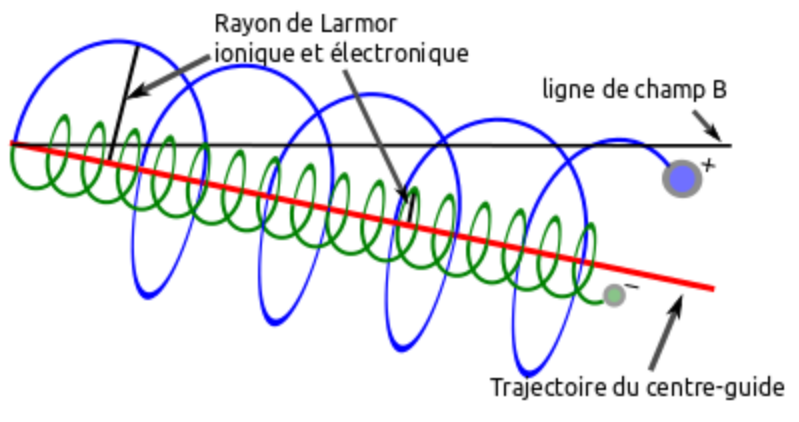
\includegraphics[width=0.8\textwidth]{figures/mouvementCyclotron.png}
{\caption{Mouvement cyclotronique des particules autour des lignes de champ
magnétique.}\label{1-particleDrifts}}
\end{figure}

(cf. figure \ref{1-particleDrifts})

\subsection{Les gaines électrostatiques}
Les gaines électrostatiques sont des structures non-neutres qui se
développent à la frontière entre un plasma et un objet. Elles apparaissent
spontanément du fait de la plus grande vitesse des électrons par rapport à
celle des ions. D'une taille de l'ordre de quelques longueurs de Debye $\lambda_D$,
L'interaction dite plasma-paroi est une branche à part entière de la physique des plasmas.
En effet, au contact d'un milieu extérieur, que ce soit un obstacle matériel
ou un gaz ambiant, le plasma perd sa quasineutralité.
\subsubsection{Physique de la prégaine}
\subsubsection{Physique de la gaine}
\subsubsection{Gaine dans les plasmas magnétisés}
\subsubsection{Problématique de la gaine parallèle aux lignes de champ}

\section{Equations fluides et phénomènes de transport}
\label{Maxwell-Boltzmann}
\subsection{De la statistique au transport fluide}
$$\partial_tf_s+\mathbf{v}_s\cdot\vec\nabla_\mathbf{r}f_s+
\frac{\mathbf{F}_s}{m_s}\cdot\vec\nabla_{\mathbf{v}_s}f_s
=\partial_tf_{|_{coll}}$$ 
Braginskii equations
$$M^{(k)}_s=\int_{-\infty}^{\infty}\mathbf{v}_s^kf_sd\mathbf{v}$$
\subsubsection{Conservation de la matière}
$$n_s=\int f_sd\mathbf{v}$$

\subsubsection{Conservation de l'impulsion}
$$n_s\mathbf{v}_s=\int \mathbf{v}_sf_sd\mathbf{v}$$
\subsubsection{Conservation de l'énergie}
\subsubsection{Conservation de la chaleur}

\subsection{Les phénomènes de transport magnétisés}
Dans un plasma collisionnel, le mouvement d'une particule peut être assimilé à
une succession de déplacements libres et de collisions, formant une marche
aléatoire de pas $\lambda_\text{lpm}$. Compte tenu du caractère isotrope du
problème, ce déplacement, sur plusieurs temps de collisions, est de
moyenne nulle. L'écart quadratique de ce déplacement à la moyenne, mesuré par la
température, ne l'est cependant pas. Il définit le processus de diffusion qui
apparaît en présence d'une inhomogénité de densité, dont la vitesse typique est
fonction de la longueur de gradient de densité et du coefficient de diffusion
$D$ :
 
\begin{equation}
    \text{V}_\text{Diff}\approx D_\alpha\frac{\nabla
    n_\alpha}{n_\alpha}=\frac{eT_\alpha}{m_\alpha\nu}\frac{\nabla
    n_\alpha}{n_\alpha}=\frac{\lambda_\text{lpm}}{L_\text{n}}v_{\text{T}_\alpha}
\end{equation}
 
où $L_\text{n}=\nabla n/n$ est la longueur de gradient de densité. 
En présence d'un champ électrique, ce déplacement aléatoire est accéléré entre
chaque collision (voir figure~\ref{1-collisions}), et entraîne un déplacement
macroscopique moyen non nul, décrit par le coefficient de mobilité :
\begin{figure}
\centering
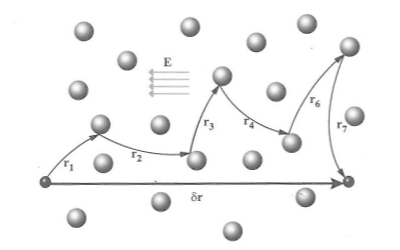
\includegraphics[width=0.8\textwidth]{figures/collisions.jpg}
{\caption{Processus de diffusion-conduction suivant la marche aléatoire
collisionnelle d'un électron~{\cite{Rax}}.}\label{1-collisions}}
\end{figure}
\begin{equation}
    \mu_\alpha=\frac{q_\alpha}{m_\alpha\nu}
\end{equation}
 
Conduction et diffusion sont les processus de transport dominants dans les
plasmas non magnétisé. Leur coefficient de transport respectifs, $D_\alpha$ et
$\mu_\alpha$, ne sont pas indépendants et leur rapport $D_\alpha/\mu_\alpha$,
appelé énergie caractéristique, est égal à la température de l'espèce selon la relation
d'Einstein :
 
\begin{equation}
    \frac{D_\alpha}{\mu_\alpha}=T_\alpha
\end{equation}
 
\section{Modèles de plasmas magnétisés}
\subsection{Les modèles numériques}
L'étude de phénomènes complexes
%\begin{figure}[htbp]
%	\centering
%	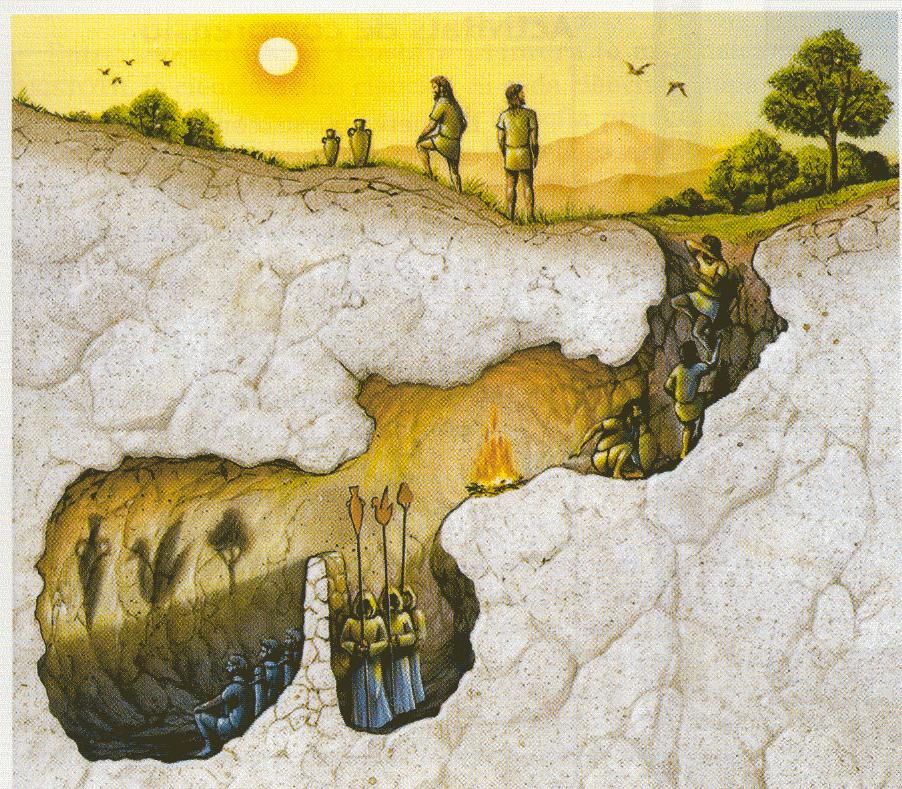
\includegraphics[height=64mm]{figures/cave.jpg}
%	{\caption{La caverne des idées.}\label{caverne}}
%\end{figure}
%\begin{figure}[htbp]
%
%			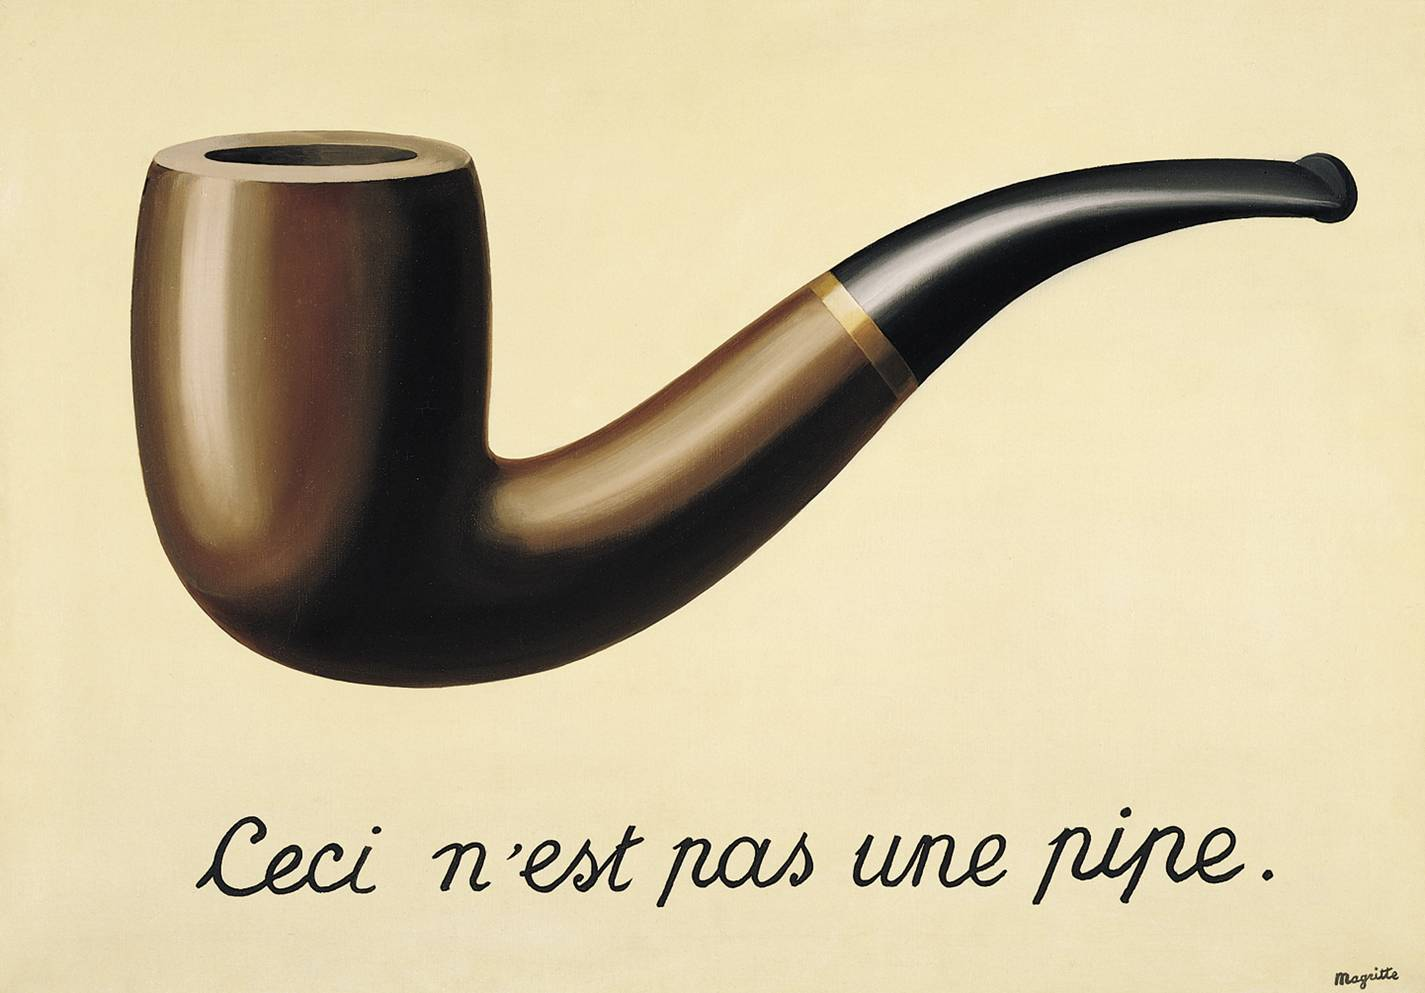
\includegraphics[height=40mm]{figures/Magritte.jpg}
%			{\caption{Magritte. La trahison des images.}\label{magritte}}
%		\end{figure}

\subsection{Les décharges plasma basse-pression}
\subsubsection{Création de la décharge, rôle des électrons}
Dans les plasmas basse-température industriels et de laboratoires, qui
possédent un faible degré d'ionisation, ou dans l'ionospère, la dynamique du
plasma est dominée par la perte de quantité de mouvement dûe à l'ionisation la force de friction avec
le gaz.
Electrical breakdown, Townsend avalanche,
\subsubsection{Transport des ions et champ ambipolaire}
\begin{equation}
\label{derivediffusion}
\end{equation}
\subsubsection{Equations de dérive-diffusion magnétisées}

\subsection{Les plasmas de bord des tokamaks}
Lawson criteriom, strongly magnetized
\subsubsection{La fusion et les tokamaks}
\subsubsection{Le plasma de la Scrape-of-Layer}
\subsubsection{Les vitesses de dérives}
\label{vitessesDerive}
%\bibliographystyle{apalike}
%\bibliography{biblio}
\end{refsection}

